%% ------------------------------------------------------------------------- %%
\chapter{Applications}
\label{cap:applications}

% \epigraph{
% Work it harder, make it better\\
% Do it faster, makes us stronger\\
% More than ever, hour after hour\\
% Work is never over}
% {Daft Punk}


%% lembrar de mencionar publicações decorrentes

% Tudo bem estar tudo em primeira pessoa do singular?

\paragraphdesc{inspiration, motivation, development, evaluation}
% The technologies evaluated during this research inspired their use in some applications.
Most of the applications presented in this chapter have been created just for case-study experiments, but others are currently helpful tools for the computer music community.
Application's open source code exemplify the use of the technologies and allow other researchers to get through code examples for getting started with MM.
The order presented here follows the application conception and the order that I was learning the technologies.
% The topics below will be presented following the conception order of the applications and the personal learning order of the technologies.

The initial motivation for these applications was indeed two courses taken during the first semester of 2012.
The first was the course of ``\textit{Computação Móvel''}~(Mobile Computing).
The professor at this time was Alfredo Goldman vel Lejbman and the Android teaching assistant was Andrew Toshiaki Nakayama Kurauchi. % this time > that time
During the course I learned the characteristics that makes Mobile Computing different from normal computing, such as the attention with the network communication, the battery consumption, and the mobility advantages. % normal computing > regular computing
I had to develop an Android application and work with delay-tolerant networking (DTN) during the discipline under the supervision of the professor and his assistant.
The classes and projects made me curious regarding the mobile technology and encouraged me to learn continuously about Mobile Computing.

% The second one (para não repetir course)
The second course was a Pure Data course ministered at ``\textit{Museu da Imagem e do Som de São Paulo} (São Paulo Museum of Image and Sound), known as MIS in São Paulo, SP, Brazil.
The professor was Alexandre Porres Torres, a member of Compmus, which was an organizer of PDcon in 2009 that happened in Brazil.
I learned the basics of Pure Data during this course and also got enchanted with the language and its possibilities.
Another point that made me interested in studying the language was the learning curve and their popularity in other fields like Music, Architecture, and Design.

After taking these two courses during the first semester of 2012, I got in contact with the book Making Musical Apps~\citep{Brinkmann2012makingmusicalapps}.
Using this book I learned how to create my first mobile application using Pure Data and Android, which is the thereminimal presented at Section~\ref{sec:appthereminimal}.
From this time on, I received other inspirations for creating new applications described in this chapter.
% Para mim tá meio exótico o "I received other inspirations". Não é melhor falar que as aplicações foram frutos de seus estudos e experimentos?

%% ------------------------------------------------------------------------- %%
\section{Android and Pure Data: thereminimal}
\label{sec:appthereminimal}

The first experiments with MM were related to user interaction through Android sensors.
These experiments resulted in a simple application inspired by the Theremin instrument which is a classical electrical instrument that presents two antennas connected to a circuit that generates audio oscillators based on the magnetic field interferences caused by musicians hands~\citep{Glinsky1992Theremin}.
% Aqui seria "controls audio oscillators" ou "generates audio waves".

The application \textit{thereminimal} is a simple application with two main files proposing the control of an oscillator with two sensors.
One sensor is selected to control the frequency and the other sensor controls the amplitude of the oscillator.
The sound synthesis used for this application was based on a Pure Data patch running with the libpd library.
The patch used in this application is presented in Figure~\ref{fig:thereminimal-pd-patch}.

The application sends the sensor's events to the Pd receivers and these values are used to control the patch variables.
The values of the sensors are converted before sending to the patch depending on each sensor.
A minimum and maximum value for pitch is defined as 200 and 2000Hz, respectively, and the volume range is from zero to one.
% A range of values for minimum and maximum pitches is defined as 200 and 2000Hz [...]
The sensor maximum and minimum values are used in this conversion based on API values sent by the API, but these minimum and maximum ranges are also updated during the audio processing in case of divergence. % 2x API
UML Class Diagram of this application is presented in Figure~\ref{fig:thereminimal-uml-classdiagram} and screenshots of the application are presented in Figure~\ref{fig:appthereminimal}.

\begin{figure}[!ht]
\centering
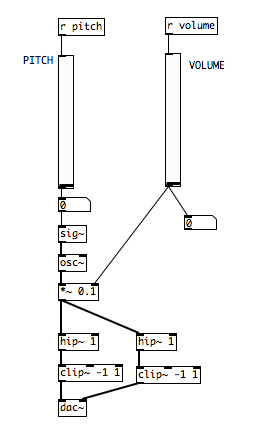
\includegraphics[width=0.3\columnwidth]{app-thereminimal-pd-patch}
\caption{Pure Data patch used in \textit{thereminimal} application.}
\label{fig:thereminimal-pd-patch}
\end{figure}

\begin{figure}[!ht]
\centering
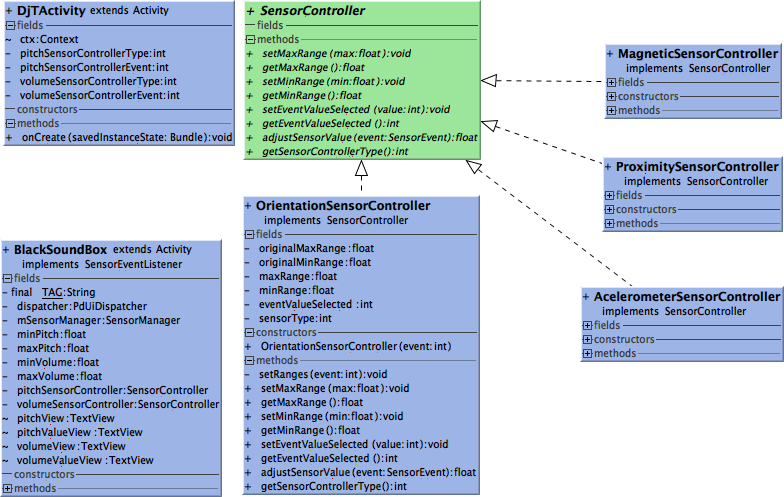
\includegraphics[width=0.9\columnwidth]{app-thereminimal-uml-classdiagram}
\caption{UML Class Diagram of \textit{thereminimal} application.}
\label{fig:thereminimal-uml-classdiagram}
\end{figure}

\begin{figure*}[!ht]
\centering
\begin{subfigure}{.30\textwidth}
	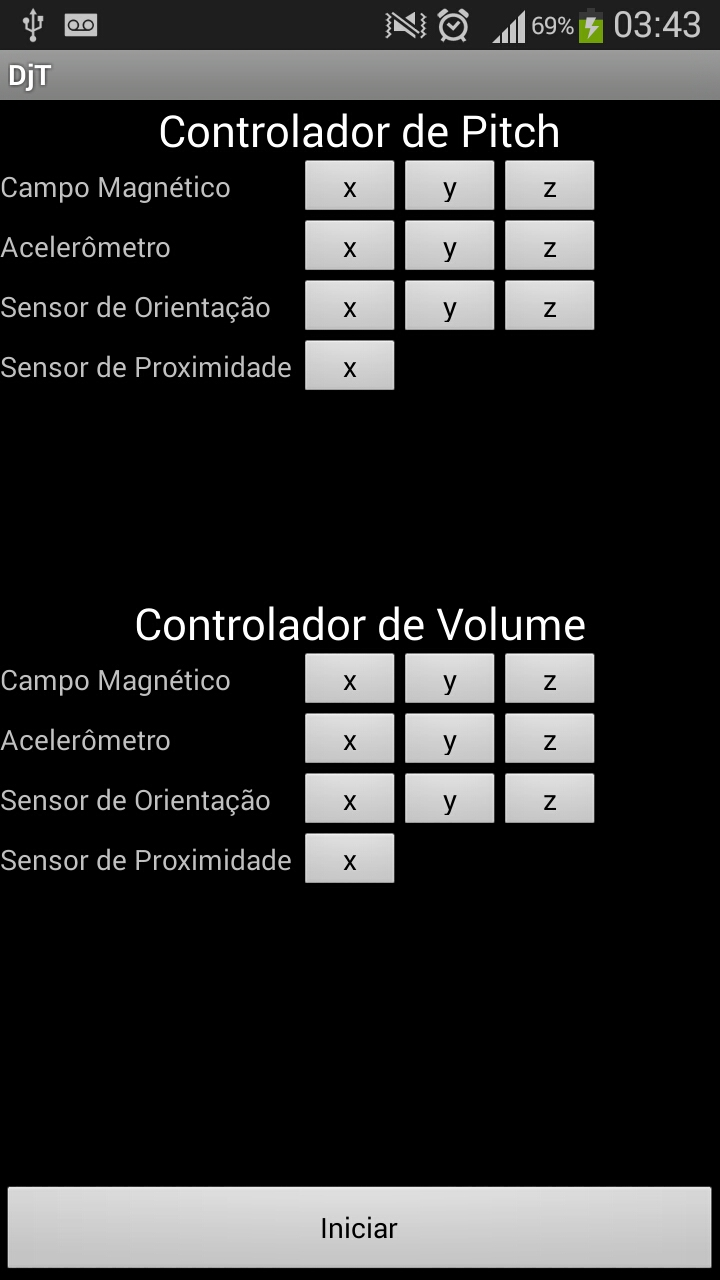
\includegraphics[width=\columnwidth]{app-thereminimal-screen1}
    \caption{First screen}
	\label{fig:appthereminimalfirstscreen}
\end{subfigure}
\begin{subfigure}{.30\textwidth}
	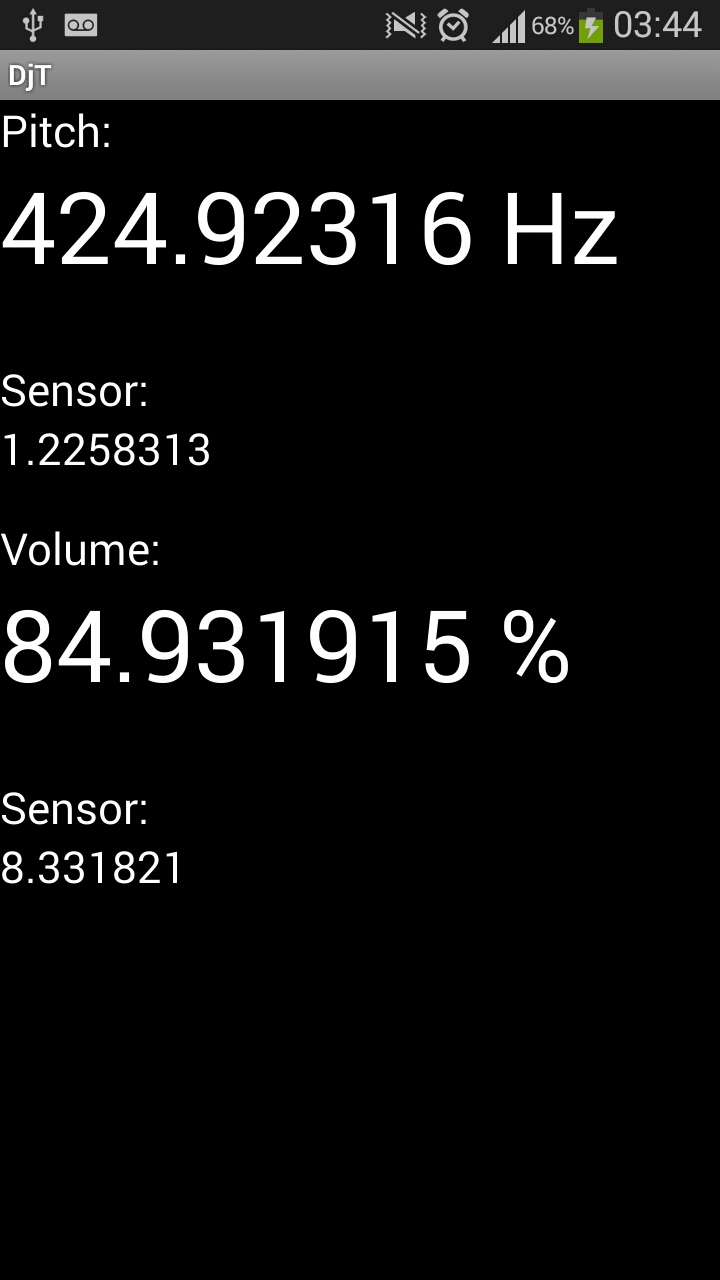
\includegraphics[width=\columnwidth]{app-thereminimal-screen2}
	\caption{Second screen}
	\label{fig:appthereminimalsecondscreen}
\end{subfigure}

\caption{Screen-shots of \textit{thereminimal} application.}
\label{fig:appthereminimal}
\end{figure*}

The first experiences with this application provided feedback regarding the Android sensor events.
Every event is captured by the API and sent to the applications that are listening to these events depending on the sample rate defined.
The fastest delay option was selected for this application, what means that the fast an event happens the fast the application will receive.
% The shortest delay option was selected by the application; this means that as soon as an event is generated, it will be received by the application.

% DJ, não entendi o que está escrito acima. Tentei ajudar no inglês, mas o significado geral não está claro para mim.
% Você quis dizer que, como o Android entrega os valores assim que eles mudam, o atraso vai ser definido pela taxa de amostragem da aplicação?
However, the variations in the values are too high that the changes in the frequencies are perceived as single separated notes instead of ramps or glissandos.
The changes in the volume are not perceived like that by most of users. % volume > amplitude

The code of the application is distributed with open source on github at the address: \url{https://github.com/deusanyjunior/thereminimal
}.
A discussion about using libpd with Android applications was presented during a talk in the regular Compmus seminars at IME-USP on October 18, 2012~\footnote{Talk about libpd and Android: \url{http://compmus.ime.usp.br/en/node/320}}.


%% ------------------------------------------------------------------------- %%
\section{Java and JNI FFT on Android: Contribution to DSPBenchmarking}
\label{sec:appdspbenchmarking}

The evaluation of audio processing on Android devices was part of the Master project conducted by the researcher Andre Bianchi at the Compmus while I was initiating my PhD research.
As soon as I learned the basics of Android application development, I started to collaborate with this project together with the researcher Max Rosan, that attended the Mobile Computing class with me.

The project evaluated many DSP methods in many Android devices focusing on the performance limits depending on the audio block size and the time required for finishing the process.
Based on the first results of this evaluation described at \cite{Bianchi2012ontheperformance}, new methods were added in order to verify the FFT performance in some variations:
% [...] verify the performance of some FFT variations:
traditional FFT, FFTW, multi-thread FFTW, double FFT, multi-thread double FFT.
While the FFTW is using JNI for calculating the FFTW coded in C language, the double FFT is based on the JTransforms library for parallel FFT calculation in Java language.

Although better performance was expected with these non-traditional approaches, running C/C++ code for small blocks increases the complexity of the application and also the cost for processing the same audio block.
A discussion regarding this evaluation was published as a paper at the 14th Brasilian Simposium of Computer Music~(SBCM) in 2013~\citep{deCarvalhoJunior2013fftbenchmark} and is presented in Appendix~\ref{ape:papersbcm2013}.

The multi-thread FFT had worst results than the traditional FFT due to Android constraints regarding the parallelism.
During this evaluation we decided to create threads using native thread methods available for Java language and these threads run in the same thread of the application as the application was requesting the threads in a wrong way.
An explanation for this behaviour is that Android programming methodologies require the use of special classes such as AsynkTask, or the packets Executor, ThreadPoolExecutor and FutureTask.
Depending on the API and the device limitations, the threads created with these solutions will provide better performance.
In this case, we found out that concurrency in Android applications is a topic that requires deep discussion and turns out to be too complex for the purpose of this research.
% Achei o trecho acima meio complicado de entender:
% Utilizar os métodos de threads nativas do Java fez com que as threads fossem criadas de forma errada? Se sim, por que?
% A exigência de utilizar AsynkTask, Executor, ThreadPoolExecutor e FutureTask foi considerada positiva ou negativa?
% Quais são as restrições do Android em relação ao paralelismo? Usar essas classes e pacotes?
% Quais são as limitações dos dispositivos? Quantidade de núcleos? Quantos GHz tem cada núcleo? Ou são limitações de software dada a versão da API?
% Mais um comentário: Um processo possui várias threads. Uma thread de um processo é executada concorrentemente com outras threads do processo.
% Então, não sei se está certo falar que "as threads rodam na mesma thread da aplicação".
% Não sei se nessa altura do campeonato eu ajudo ou atrapalho com comentários assim, mas achei importante chamar a atenção.


The code of the application is distributed with open source on github at the address:~\url{https://github.com/andrejb/DspBenchmarking}.

%% ------------------------------------------------------------------------- %%
\section{Android, CSound, and RoR: Touches On The Line}
\label{sec:apptouchesontheline}

The first attempt to create collaborative applications for Mobile Music was through the use of a web service programmed using Ruby on Rails.
The idea of creating a web service was the first idea for this solution considering my personal background as web developer.
The technologies selected were based on the recent technologies learned at this time. % 2x technologies
                                                                         % that?
In 2012 I attended the Mobile Computing course and I was admitted as Teaching Assistant for the same course in the next two years.
% ^ já falou lá em cima que fez a disciplina! ;-)
During this period I had to create many web services for the assignments proposed to the students and I had to choose a platform available for rapid application development~(RAD).
The Ruby on Rails~(RoR) was one of the available options at this time that caught the attentions due to its simplistic way to create online solutions. % this time > that time
An advantage for this solution is also that the POST and GET requests using JSON format were added to the web service with few lines of code.
% Another advantage for this solution is that [...]

The CSound portability for Android devices was published on Linux Audio Conference in 2012~\citep{Yi2012csound}.
This paper inspired the use of CSound for mobile applications as it presented many samples using diverse approaches for interaction through Android inputs and CSound scores.
% This paper inspired the use of CSound for mobile applications because it presented many examples using numerous approaches [...]          
The \textit{MultiTouchXY}~\footnote{MultiTouchXY code: \url{https://github.com/csound/csound/blob/develop/android/CsoundAndroidExamples/src/com/csounds/examples/tests/MultiTouchXYActivity.java}} application was selected as a starting point for the development of \textit{Touches On The Line} application due to the high sample rate of events available from touch events.
Touch responsiveness on Android devices can have values up to 120~Hz and provides up to 10 fingers position, what implies 10 pair of position values~(x and y) on every 8~ms in the best situation~\cite{Padre2017touchresponsiveness}.

\textit{Touches On The Line} application was defined as an application proposed to share touch's movements online and have its position synthesized as sound.
% 2x application
% Acho que pode remover o "proposed"
The \textit{MultiTouchXY} demo application was provided with a CSound score that receives two values and control a sound synthesis varying frequency and timber~\footnote{MultiTouchXY score for CSound: \url{https://github.com/csound/csound/blob/develop/android/CsoundAndroidExamples/res/raw/multitouch_xy.csd}}.
The demo was first changed to send every new event to the web server, and in the background the application would request new available values from the server.
This approach was changed even during the development due to many reasons: the communication with the web server was taking too long; the application was getting
unresponsive in case many touch events were sent at the same time, due to many posts running in background;
% unresponsive when many touch events [...]
and the touch events were posted too fast so the request for new available data were receiving many new data for every request.

% Tem uma coisa que não ficou clara para mim, então acho que cabe uma refatoração no texto acima para ajudar outros leitores.
% Temos diversos eventos cada um gerando um POST (e o problema é na quantidade de requisições)?
% Ou temos vários eventos sendo acumulados em um POST gigante (e o problema está no tempo de resposta)?
% Quando você fala "the touch events are posted too fast" interpreto a primeira coisa.
% Quando você fala "many touch events were being sent at the same time" interpreto a segunda coisa.
% Ainda, acho que a frase "posts running in background" não está 100% certa. São os processos que fazem as requisições HTTP POST que estão se acumulando em bg, certo?

The latest version of this application was developed with a buffer for a touch movement from the time the finger touches the screen to the release, including the delay between each timestamp received with the finger event.
% Daqui para baixo me perdi com o que você chamou de delay. Existe um atraso na captura dos eventos de touch? Ou você quis falar apenas do intervalo de tempo que
% a pessoa demorou para ir de um ponto a outro no path? Se for a duração da transição entre pontos, recomendo fazer um 's/delay/interval/g'. ;-)
The finger movement is reproduced on the local device sending every new event to the CSound synthesizer, and the complete movement is then sent to the web service after releasing the finger from the screen.
This data is exchanged with the web service using JSON format and contains only float numbers for position and integer numbers for delays in milliseconds.

Although this application allows many devices to participate in the same session, it was evaluated only with three devices available at lab during the period of its conception.
After its development, the application was used in some solo performances and experienced by many users during talks and presentations without problems for music interaction.
A log with all events sent through the application is available online through the main page of the web application at \url{http://wscompmus.deusanyjunior.dj/cscores}.
An example of an event is presented below:

\begin{itemize}\itemsep0em
\item[] [4873] [2013-10-27 11:15:27 UTC] userid: 79 - score: s 0,168750 0,181234;d1;m13 0,166667 0,181234;m17 0,166667 0,181234;m72 0,172917 0,181234;m12 0,172917 0,181234;m17 0,172917 0,181234;m17 0,172917 0,181234;u16;
\end{itemize}

This event includes the timestamp of received event, the random identification selected for the user from the application, and the score.
The score initiates with the xy initial position of the finger, includes the required delay applied before using the next finger position before each other finger position, and finishes with the delay before releasing the finger.

The development of Android applications with CSound was the topic of a talk during the regular seminars of Compmus at IME-USP, on October 1st, 2013~\footnote{Talk about Android and CSound: \url{http://compmus.ime.usp.br/en/node/377}}.
The application was published as a technical paper at 2nd International Conference in 2013~\citep{deCarvalhoJunior2013touches} and is presented in Appendix~\ref{ape:papericsc2013}.


%% ------------------------------------------------------------------------- %%
\section{Android and Sensors: Sensors2}
\label{sec:appsensors2}

% The creation of the \textit{thereminimal} provided the necessary code for any person with minimum knowledge about Android programming to use the Android sensors.
Using the Android sensors for creating the \textit{thereminimal} provided the necessary code for any person with minimum knowledge about Android programming.
However, some users would find it still hard to take advantage of all Android sensors in this case. % some users found?
The idea of creating an Android application that could make the use of Android sensors feasible started with Sensors2Pd and extended to Sensors2OSC, resulting in the conception of Sensors2~\footnote{Sensors2 web site: \url{sensors2.org}} in a partnership with Thomas Mayer from Residuum.

The idea behind Sensors2 is to develop mobile applications that can help users to use Android sensors with many other technologies.
\textit{Sensors2Pd} aims the use of Android sensors with Pure Data patches that can be loaded on the application.
\textit{Sensors2OSC} sends Android sensors through the network using OSC format.
\textit{Sensors2Log} is an application that can save the sensors inputs to files inside device's internal or external memory.
The applications are being distributed through the F-Droid~\footnote{F-Droid website: \url{https://f-droid.org/}} platform as well as through the github.
A description of the development process of each application is present below.

%%%%%%%%
\subsection*{Sensors2Pd}
\label{subsec:appsensors2pd}

Many mobile applications were developed in order to turn the mobile device into an instrument just as discussed in Section~\ref{sec:mobileinstruments}.
Additionally, some applications provided the option to use Android sensors for music interaction, such as urMus, Control, and MobMuPlat.
The main restriction of these applications is that they support only few sensors, while Android sensor options are increasing through the time.
Based on this condition, \textit{Sensors2Pd} was created following an approach that is able to support all current and future Android sensors.

The idea behind \textit{Sensors2Pd} comes from the Android Sensors API~\footnote{Android Sensors API header file from repository: \url{https://android.googlesource.com/platform/hardware/libhardware/+/master/include/hardware/sensors.h}}.
Every type of sensor is registered at the API with an integer number.
A list of these sensors and IDs is presented at Appendix~\ref{ape:android-sensors}.
The sensor manager used on Android applications provides a listener which informs the sensor ID and the latest values from an event received by a sensor. % by it?
Although it is possible to register for receiving only the data regarding a specific sensor, the API offers the option to receive information regarding all sensors.
% Although it is possible to register to receive only [...]
In this case, \textit{Sensors2Pd} provides an interface for sending the sensor's events to receivers at Pure Data patches using that need to follow the pattern:
% In this case, \textit{Sensors2Pd} provides an interface to send the sensor's events [...]
% Não consegui entender o finalzinho da frase: "using that need to follow the pattern".

\begin{itemize}\itemsep0em
\item[] [receiver sensor\{ID\}v\{\#\}]
\end{itemize}

The ID represents the sensor ID from the API documentation, and the \# is the index of the event variable.
Considering the accelerometer sensor that has the ID=1 and presents 3 variables representing the x, y, and z coordinates, the user needs to add the following receivers:

\begin{itemize}\itemsep0em
\item[]    [receiver sensor1v0]
\item[]    [receiver sensor1v1]
\item[]    [receiver sensor1v2]
\end{itemize}

The application was programmed to send the values in a loop.
This loop creates the messages automatically and send them based on the values that come from the API.
This approach allowed the \textit{Sensors2Pd} to be compatible with all available sensors at an Android device as long as the API continues with the same strategy.

Touch position is sent to Pure Data patches following a similar approach.
The Android system offers a listener for touches that reports the x and y position of the touch on the screen including an ID for each finger.
The IDs varies from 0 to 14, although Android devices support up to 10 touches.
A finger receives an ID as soon as it is recognized on the screen, and these IDs start with 0 increasing as new fingertips are recognized.
In case a finger is released and other fingers are still touching the screen, the next finger touching the screen will get the next available ID between 0 and 14.
The receivers used for touches follow the pattern:

\begin{itemize}\itemsep0em
\item[]  [receiver sensorT{ID}v{\#}]
\end{itemize}

The ID represents the finger ID defined by the Android API, while the \# represents the coordinate.
An example of receivers for the finger with ID=0 are presented below:

\begin{itemize}\itemsep0em
\item[]   [receiver sensorT0vx]
\item[]   [receiver sensorT0vy]
\end{itemize}

Another sensor available at Sensors2Pd is the WiFi sensor.
The Android API offers a lot of information regarding all available networks, such as SSID, BSSID, frequency, and signal level in dBm.
In this case, the application sends SSID's level to Pd patches.
The user needs to configure the receiver following the pattern:

\begin{itemize}\itemsep0em
\item[]    [receiver sensorW-{SSID}]
\end{itemize}

% When the WiFi SSID is [...]
In case the WiFi SSID is "MyRouter", the receiver needs to be:

\begin{itemize}\itemsep0em
\item[]    [r sensorW-MyRouter]
\end{itemize}

% 2x "The application" - Você poderia tirar o ponto-final e escrever "and its code" (não esquecendo de ajeitar o outro "and" mais para frente).
The application was presented during the regular talks from Compmus at IME-USP on August 25th, 2014~\footnote{Talk about Sensors2Pd: \url{http://compmus.ime.usp.br/en/node/432}}.
The application code can be found at \url{https://github.com/SensorApps/Sensors2Pd} and was used during the development of the project Hoketus described at Section \ref{sec:apphoketus}.
This application was published as a paper at the Joint Conference of the 40th International Computer Music Conference and 11th Sound and Music Computing Conference, Athens, Greece, in 2014~\citep{deCarvalhoJunior2014sensors2pd}.
This paper is presented at Appendix~\ref{ape:papericmc2014}.

%%%%%%%%
\subsection*{Sensors2OSC}
\label{subsec:appsensors2osc}

The development of \textit{Sensors2OSC} followed a strategy similar to the one applied during the development of \textit{Sensors2Pd}.
The application adapts to the available sensors at any Android device without restricting the use of new sensors that may become available.
Sensor events are converted to OSC messages and sent through UDP to a IP and Port specified by the user on the settings screen of this application.
The namespaces used for sending OSC messages have been updated for some sensors.
Table~\ref{tab:mapping} with current personalized OSC prefixes.
New sensors receive the prefix based on sensor ID, as for example the new sensor with ID=30 that receives the prefix /30.
% New sensors receive the prefix based on its ID. For instance, a new sensor with ID=30 will receive the prefix /30.

\begin{table}[t]
\centering
\caption{Mapping from Android sensors to OSC messages in Sensors2OSC}
\label{tab:mapping}
\begin{tabular}{|l|l|l|}  \hline
ID & OSC prefix                  & Dimensions \\   \hline
1  & \lstinline$accelerometer$             & 3          \\
2  & \lstinline$magneticfield$             & 3          \\
3  & \lstinline$orientation$              & 3          \\
4  & \lstinline$gyroscope$                 & 3          \\
5  & \lstinline$light$                      & 1          \\
6  & \lstinline$pressure$                   & 1          \\
7  & \lstinline$temperature$                & 1          \\
8  & \lstinline$proximity$                  & 1          \\
9  & \lstinline$gravity$                   & 3          \\
10 & \lstinline$linearacceleration$        & 3          \\
11 & \lstinline$rotationvector$            & 4          \\
12 & \lstinline$relativehumidity$           & 1          \\
13 & \lstinline$ambienttemperature$         & 1          \\
14 & \lstinline$magneticfielduncalibrated$  & 6          \\
15 & \lstinline$gamerotationvector$        & 3          \\
16 & \lstinline$gyroscopeuncalibrated$     & 6          \\
17 & \lstinline$significantmotion$          & 1          \\
18 & \lstinline$stepdetector$               & 1          \\
19 & \lstinline$stepcounter$                & 1          \\
20 & \lstinline$georotationvector$         & 4          \\
21 & \lstinline$heartrate$                  & 1         \\ 
22 & \lstinline$tiltdetector$               & 1      \\
23 & \lstinline$wakegesture$             & 1      \\
24 & \lstinline$glancegesture$           & 1      \\
25 & \lstinline$pickupgesture$           & 1     \\ \hline
\end{tabular}
\end{table}

The first design of \textit{Sensors2OSC} had the option to select the coordinates of each sensor that would be sent through OSC, as presented in Figure~\ref{fig:appsensors2oscfirstdesign}.
In this case, one OSC message would be sent for every coordinate selected.
Some users reported that this approach was blocking them from using the application for controlling 3D objects as the UDP messages are not sequentially received and they can be lost even on local networks.
These reports led to an update on the application in which the user selects only the sensor instead of its variables.
The current version of \textit{Sensors2OSC} packs all values and send them in a single OSC message, and its design is presented in Figure~\ref{fig:appsensors2oscseconddesign}.

\begin{figure*}[!ht]
\centering
\begin{subfigure}{.30\textwidth}
	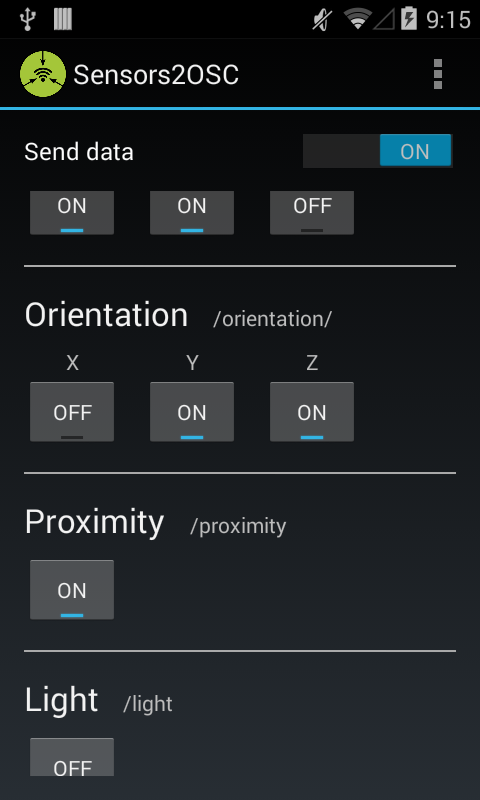
\includegraphics[width=\columnwidth]{osc_main}
    \caption{First screen design}
	\label{fig:appsensors2oscfirstdesign}
\end{subfigure}
\begin{subfigure}{.28\textwidth}
	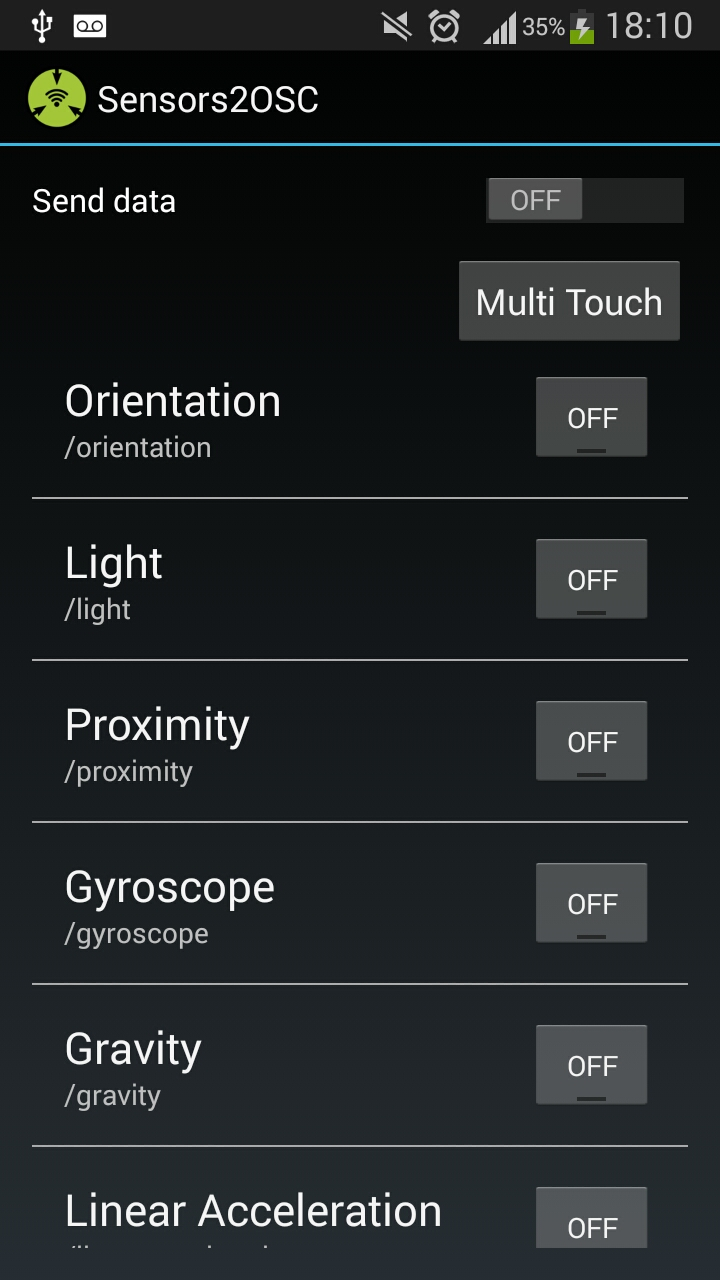
\includegraphics[width=\columnwidth]{osc_main_new}
	\caption{Current design}
	\label{fig:appsensors2oscseconddesign}
\end{subfigure}

\caption{Screen-shots of \textit{Sensors2OSC} main screen designs.}
\label{fig:sensors2oscmainscreen}
\end{figure*}

The application has been used by Thomas Mayer in many of his performances, and I used this application in the performance \textit{AntonioZ} at \textit{Concertos de Computação Musical}~(Computer Music Concerts)~\footnote{Concerts description: \url{http://prceu.usp.br/semanadearteecultura/evento/concertos-computacao-musical/}} organized by me in 2016 at the IME-USP during \textit{Semana de Arte e Cultura da USP}~(Art and Culture Week from USP).
Other users have reported the use of this application and requested modifications.
Mladen Radolovic is a Croatian user that requested the addition of an option to send NFC tags' information through OSC and now the application is able to send the NFC tags identification through the namespace /nfc.
Tal Kirshboim is a German user that included the Multitouch option on the application and continue debugging the code. % and he continues to debug the code
A user from Japan also contributed with the translation of the application to Japanese, and now the application is internationalized to four languages including English, German, and Portuguese.

A discussion about mapping Android sensors using OSC on Android devices with this application was presented during a talk in the regular Compmus seminars at IME-USP on June 29th, 2015~\footnote{Talk about mapping Android sensors to OSC: \url{http://compmus.ime.usp.br/en/node/465}}.
The application code can be found at \url{https://github.com/SensorApps/Sensors2OSC}.
This application was published as paper at the Sound and Music Computing Conference at Maynooth, Ireland, in 2015~\citep{deCarvalhoJunior2015sensors2osc}.
This paper is presented at Appendix~\ref{ape:papersmc2015}.

%%%%%%%%
\subsection*{Sensors2Log}
\label{subsec:appsensors2log}

During the experiences with these applications I was invited to work in a project related to patient monitoring. % paciente de que? apneia?
The main intention of this project was to register information of a person while sleeping.
This data would be analyzed by computer programs and diagnose person's healthy afterwards.
% The main goal of this project was to diagnose a person's health by analising the data registered while he/she is sleeping.
The code of Sensors2Pd was then changed to record the sensors values to files instead of sending to Pure Data patches.
Another feature of this project was the audio recording into MP3 and WAVE formats.

The current application is still under development, but it has been tested in many different situations.
The first evaluation was for monitoring a patient in \textit{Laboratório do Sono}~(Sleep Lab) at \textit{Instituto do Coração}~(Heart Institute) from USP.
% A strap was designed [...]
A strap was projected to hold the mobile device over the body of a patient and allow the device to be in the same position of the patient.
Audio and sensors were registered during a whole night of sleeping.
The data was then retrieved from the mobile device through the internal memory using the USB cable and evaluated by many programs on Desktop computers.
Other evaluations were conducted to register the sensor values and verify movements accuracy with success.
% "resulted in results" / melhor colocar "provided" ou "generated"
The use of this application resulted in many interesting results regarding Android sensors.
% Although the application recorded [...]
Although the application was recording data for more than 10~hours in a row, the battery consumption was less than 50~\% in a Sony Xperia Play smartphone with the screen turned off during the evaluation.

After the experiments, the application was dubbed \textit{Sensors2Log} and aggregated to the \textit{Sensors2} collection.
The application can be used in many monitoring process with options for selecting the sensors and the audio recording settings.
Figure~\ref{fig:sensors2log} shows two screens of the application and the current application code can be found at \url{https://github.com/SensorApps/Sensors2Log}.

\begin{figure*}[!ht]
\centering
\begin{subfigure}{.35\textwidth}
	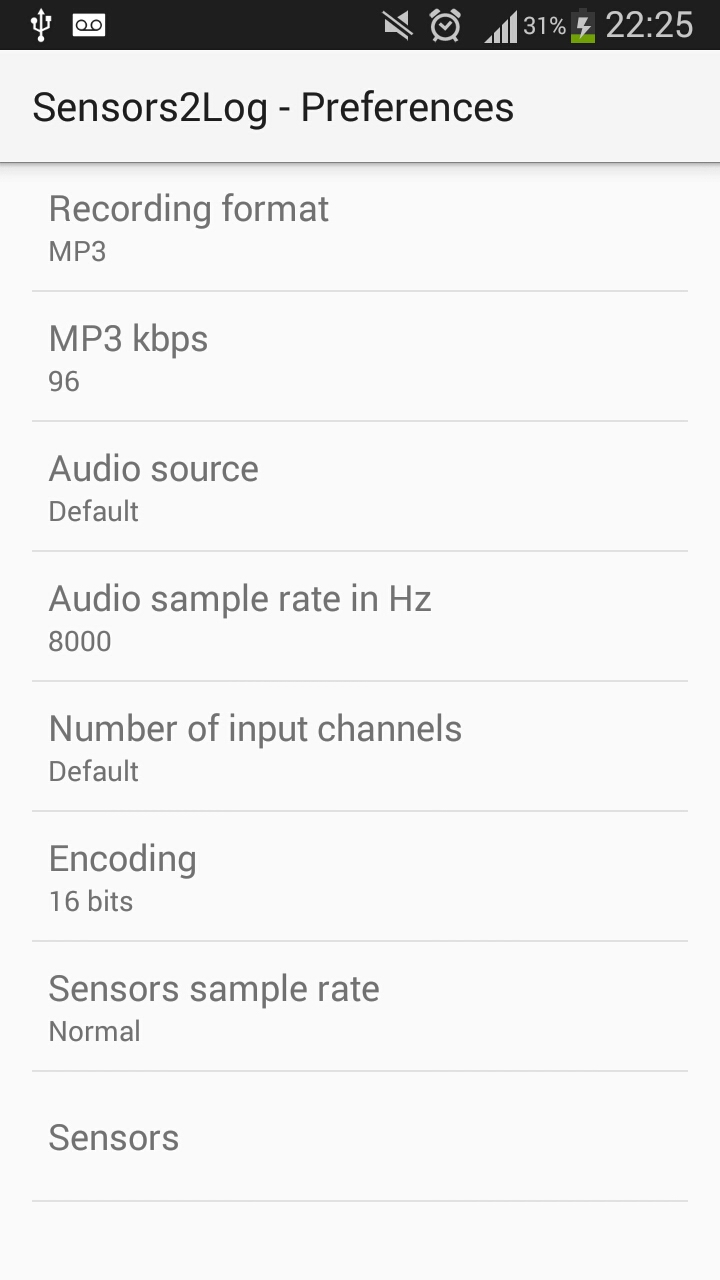
\includegraphics[width=\columnwidth]{sensors2log_screenshot1}
    \caption{Preferences screen}
	\label{fig:appsensors2log1}
\end{subfigure}
\begin{subfigure}{.35\textwidth}
	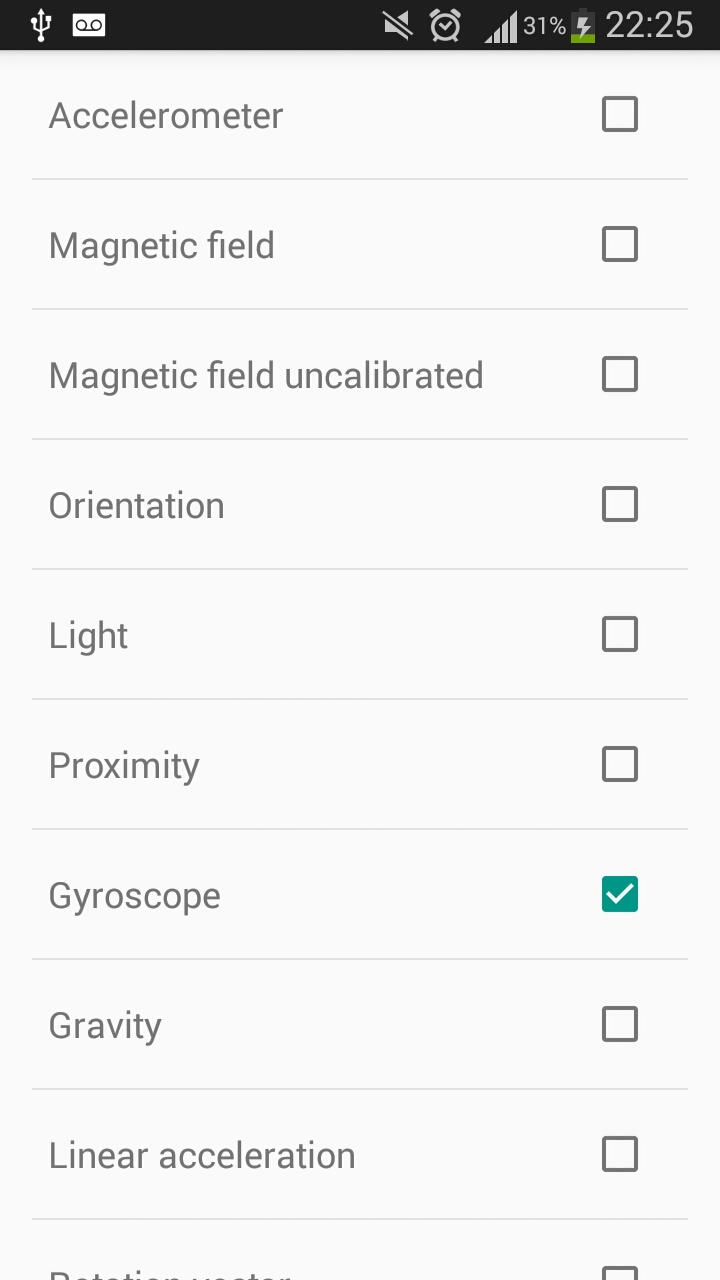
\includegraphics[width=\columnwidth]{sensors2log_screenshot2}
	\caption{Sensor selection screen}
	\label{fig:appsensors2log2}
\end{subfigure}

\caption{Screen-shots of \textit{Sensors2Log}.}
\label{fig:sensors2log}
\end{figure*}


%% ------------------------------------------------------------------------- %%
\section{Indoor localization and Pure Data: Hoketus installation}
\label{sec:apphoketus}

The code of \textit{Sensors2Pd} was used to create the application \textit{Hokeuts} during an installation under the same name.
This installation took advantage of the WiFi level to identify users close to specific routers.
The application was created with the Sensors2Pd code embedded and the application interface was personalized especially for this installation. 

Some smartphones were configured as hotspots and the Pure Data patches created for this installation were defined to synthesize different sounds depending on the SSID found.
The participants were invited to install an application that would find hotspots and also synthesize different sounds.
A web server was set up using the same technologies and approaches presented in Section~\ref{sec:apptouchesontheline} but with specific pages for each hotspot.
The participants' application had a method to send the level of the SSID found to the web service, and the hotspots' application were configured to request the SSIDs' level in order to amplify their synthesis depending on the number of close devices.

During the performance, the hotspots used the 3G interface to connect to the Internet, since the Wi-Fi interface was being used as a hotspot antenna. 
It is important to notice that the participants were possibly using the 3G data connection and nobody reported any issue regarding the consumption of the 3G plan during the performance.
Most of the questions regarding the installation were related to interaction aspects that were somewhat incomprehensible at some locations.
The Figure \ref{fig:installation} represents the installation with the hotspots and the participants while Figure \ref{fig:installation-schema} shows an example of network communication between the mobile devices. 
In both images the hotspots have a circle representing their best signal strength area.

\begin{figure*}[!ht]
\centering
\begin{subfigure}{.45\textwidth}
	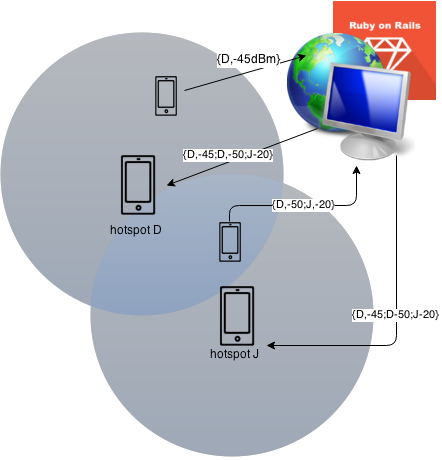
\includegraphics[width=.90\columnwidth]{nime2015-schema}
    \caption{Network communication}
	\label{fig:installation}
\end{subfigure}
\begin{subfigure}{.45\textwidth}
	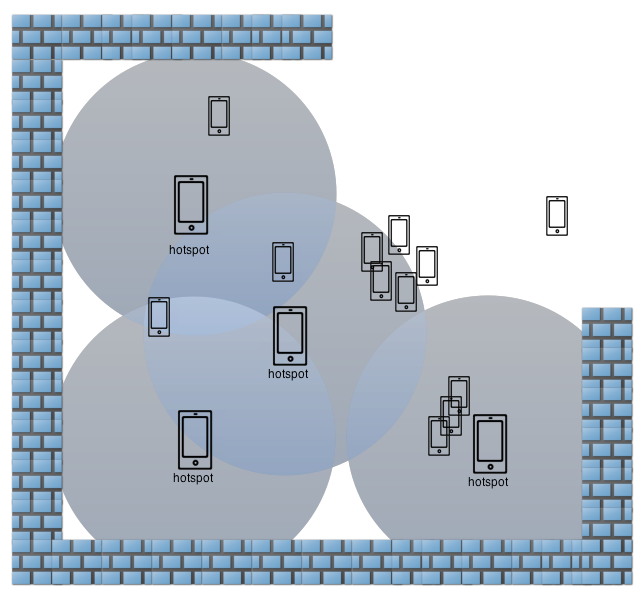
\includegraphics[width=\columnwidth]{nime2015-installation}
	\caption{Four hotspots installation}
	\label{fig:installation-schema}
\end{subfigure}

\caption{Hoketus installation.}
\label{fig:hoketusinstallation}
\end{figure*}

An aesthetic discussion about this installation and other experiences with Sensors2PD can be found at the paper presented at The Fourteenth Biennial Symposium on Arts and Technology, Connecticut College, New London, CT, USA, in 2014~\citep{Bandeira2014notes}.
A discussion about the advantage of using WiFi for indoor localization with this application during the Hoketus project was published as a paper and presented as a poster during at the International Conference on New Interfaces for Musical Expression, Baton Rouge, Lousianna, USA, in 2015~\citep{deCarvalhoJunior2015indoor}.
These papers are presented at Appendix~\ref{ape:paperbats2014} and Appendix~\ref{ape:papernime2015}, respectively.
The code used on \textit{Hoketus} mobile application is available at \url{https://github.com/deusanyjunior/hoketus}.


%% ------------------------------------------------------------------------- %%
\section{Network evaluation on Android: PushLoop}
\label{sec:apppushloop}

During this research, many network technologies were evaluated through a simple application.
The code of this application was organized to work as an example of how user can communicate through the network options selected and the whole codification was simplified by its maximum.
The main intention was is to provide an easy way to exchange messages between mobile devices around the world with minimum codification effort.
The application created for this evaluation was named PushLoop and included settings for evaluating Unicast IPv4, Unicast IPv6, Multicast, and Cloud Services.

PushLoop Android application is based on the loop-back concept, so one device would send messages, the ``\textit{sender}'', while the other device, the ``\textit{loopback}'', would answer the message as soon as possible, simulating a loop-back circuit.
The first device registered all messages sent and received on a report file with millisecond time-stamp precision.
The method used to register the events on the report was \textit{SystemClock.elapsedRealtime()}.
We also run AsyncTask invoking \textit{executeOnExecutor()} with \textit{THREAD\_POOL\_EXECUTOR} in order to have parallel execution on Android.
The messages had five divisions: a unique device id; message number with cycle number on the range of thousands; the total number of messages; a random integer as a key for message identification; and a block of floats.
An example of a message used during the tests is presented below:

\begin{footnotesize}
\begin{center}
23.0.1.A87422113 1001 1000 76 [0.28506452]
\end{center}
\end{footnotesize}

An activity diagram is presented on Figure~\ref{fig:pushloopactivityDiagram} representing the point of view of a sender activity on the application.
The class diagram is presented on Figure~\ref{fig:pushloopclassdiagram}.
This diagram includes all class from the current version of the application after many changes during the development process due to network experimentation.
Screenshots of the PushLoop application are presented on Figure~\ref{fig:pushloopscreenshots}.

\begin{figure}[!ht]
\centering
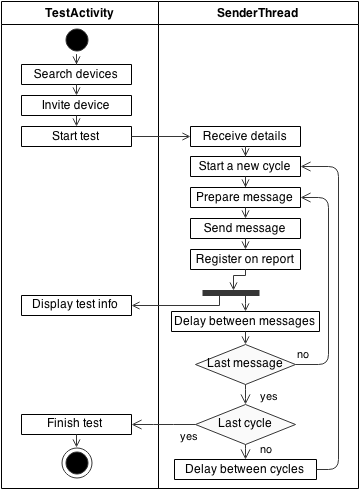
\includegraphics[width=0.40\columnwidth]{testActivityDiagram-BW}
\caption{PushLoop activity diagram of the test from the sender point of view.}
\label{fig:pushloopactivityDiagram}
\end{figure}

\begin{figure}[!ht]
\centering
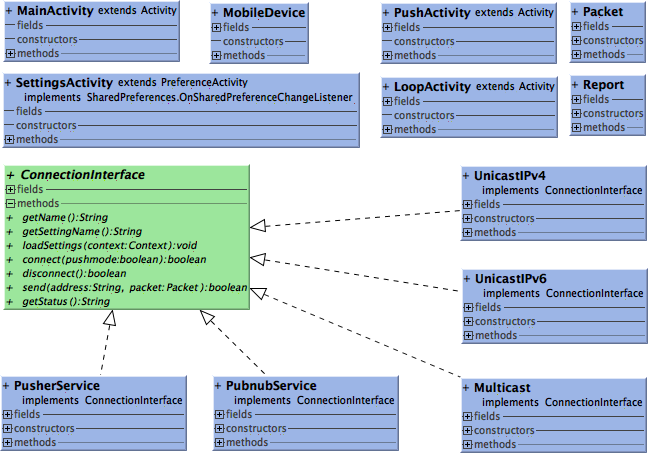
\includegraphics[width=\columnwidth]{PushLoop_ClassDiagram}
\caption{PushLoop class diagram.}
\label{fig:pushloopclassdiagram}
\end{figure}

\begin{figure*}[!ht]
\centering
\begin{subfigure}{.20\textwidth}
	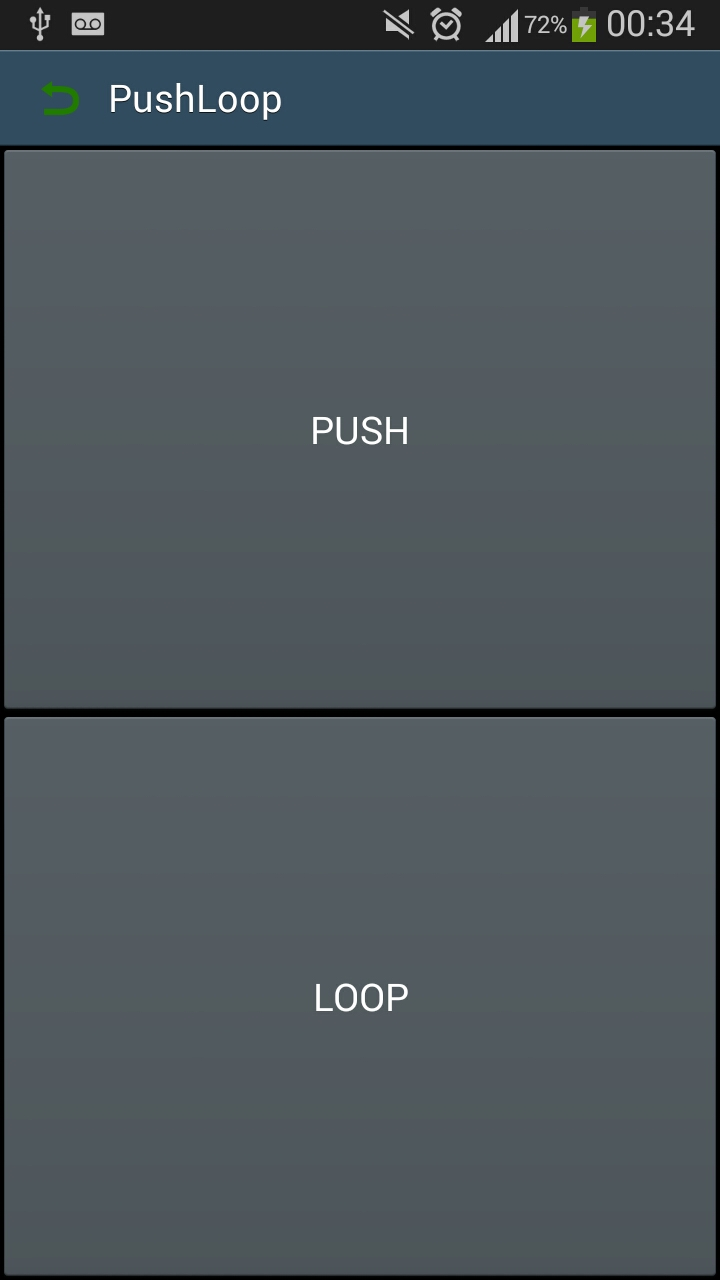
\includegraphics[width=\columnwidth]{pushloop_screenshot}
    \caption{Main screen}
	\label{fig:pushloopss1}
\end{subfigure}
\begin{subfigure}{.20\textwidth}
	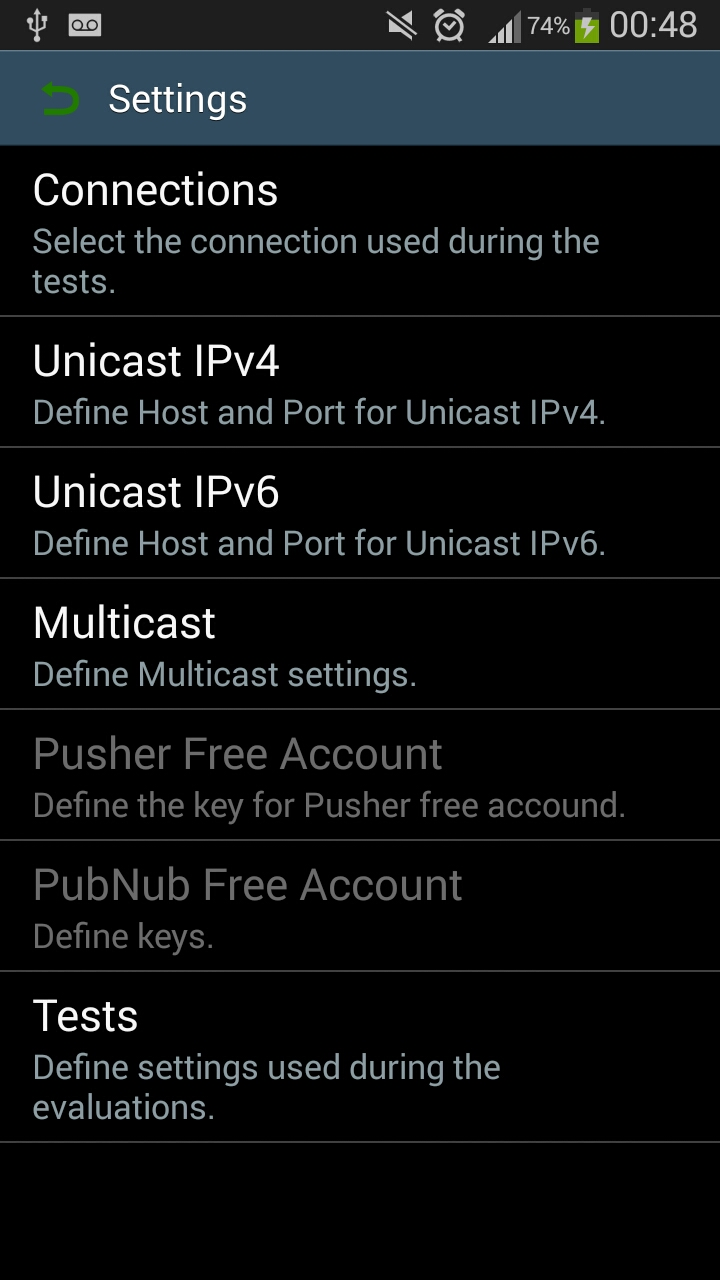
\includegraphics[width=\columnwidth]{pushloop_screenshot2}
	\caption{Settings screen}
	\label{fig:pushloopss2}
\end{subfigure}
\begin{subfigure}{.20\textwidth}
	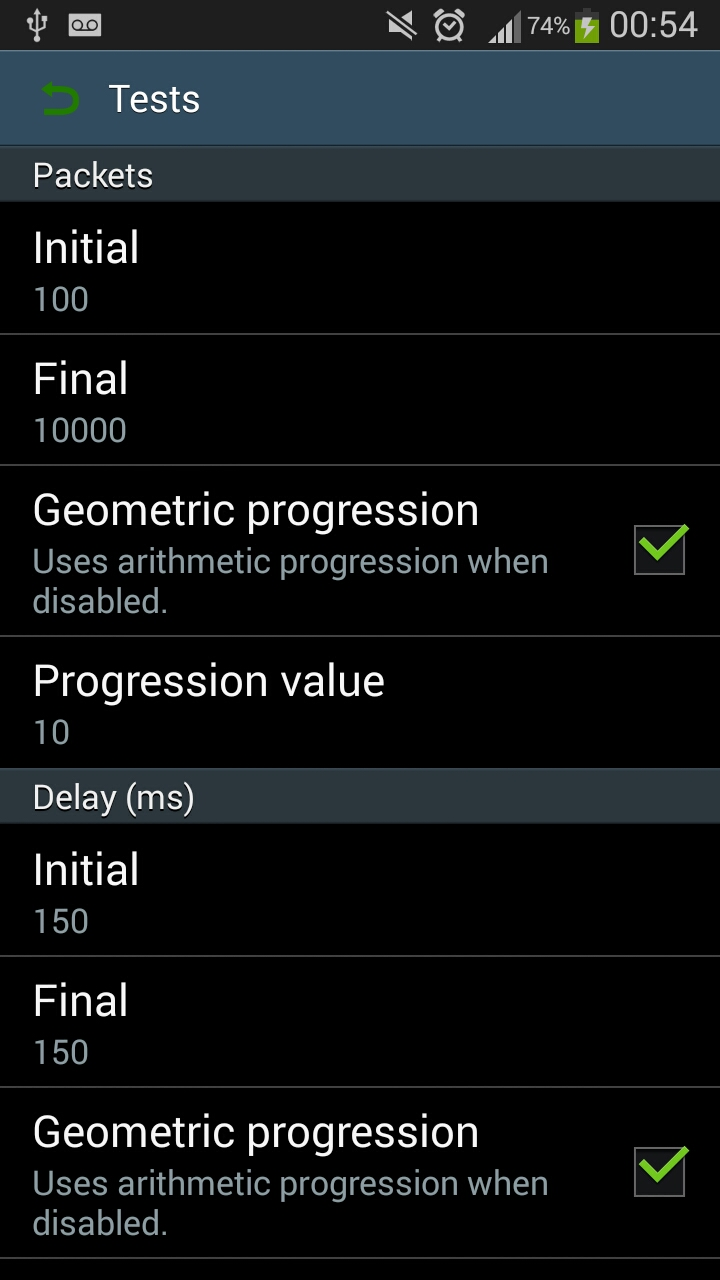
\includegraphics[width=\columnwidth]{pushloop_screenshot3}
	\caption{Test settings screen}
	\label{fig:pushloopss3}
\end{subfigure}
\begin{subfigure}{.20\textwidth}
	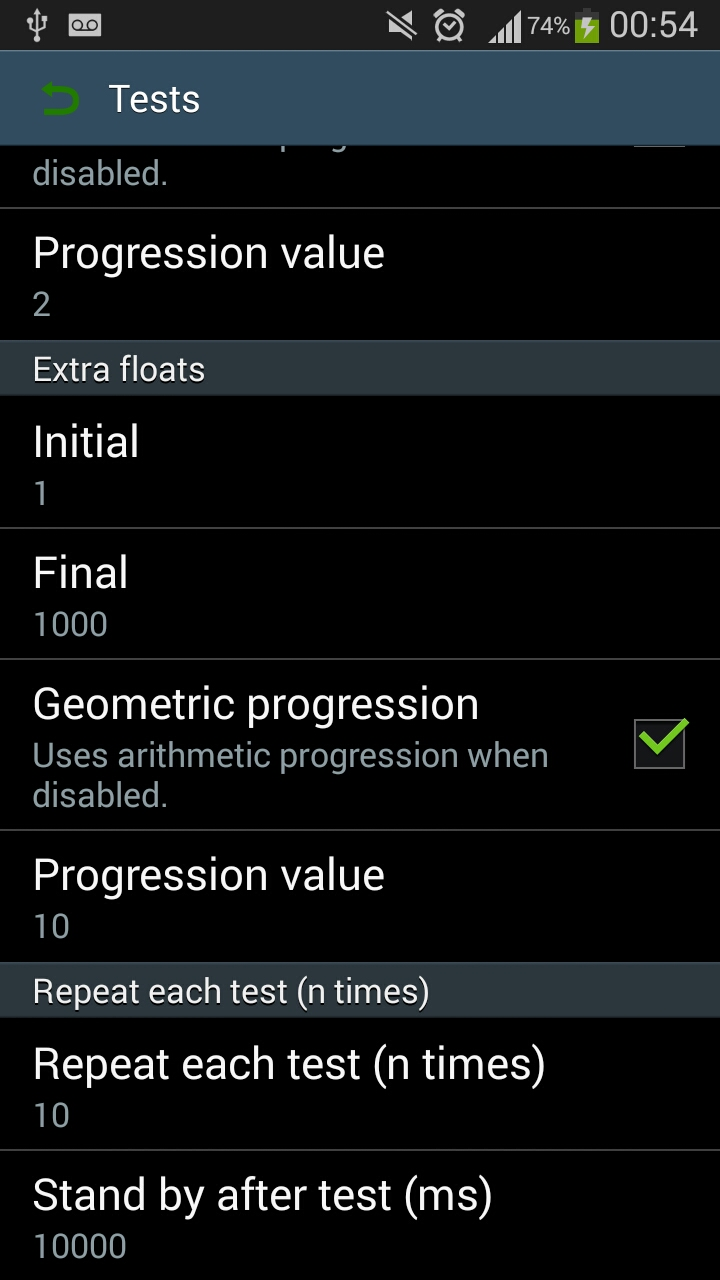
\includegraphics[width=\columnwidth]{pushloop_screenshot4}
	\caption{Test settings screen continuation}
	\label{fig:pushloopss4}
\end{subfigure}

\caption{PushLoop application screenshots.}
\label{fig:pushloopscreenshots}
\end{figure*}

The code of the application is available at \url{https://github.com/deusanyjunior/PushLoop}. 
The first evaluation using this application was published as a paper at the International Computer Music Conference, 2015, Denton, Texas, in 2015~\citep{deCarvalhoJunior2015computer}.
This paper is presented at Appendix~\ref{ape:papericmc2015}.
The Chapter~\ref{cap:evaluations} is based on the evaluations conducted with this application.


%% ------------------------------------------------------------------------- %%
\section{Cloud Services for presentations: pubslides}
\label{sec:apppubslides}

One of the first simple and useful application created with the use of Cloud Services during this research was the \textit{pubslides}.
This application was made with HTML, CSS, and Javascript with the aim of sharing the current slide page with the audience during a presentation.
The person that is giving a talk can control the current slide position from the master page of \textit{pubslides}, while the other users follow the presentation on the client page.

The process for adapting any presentation to this application is also simple.
The \textit{pubslides} code needs to be available at some web server accessible by the audience from the Internet, the presenter needs to open the master page presented on Figure~\ref{fig:pubslidesmaster}, and the the audience needs to open the index page presented on Figure~\ref{fig:pubslidesclient}.
The current version of pubslides require the PDF to be converted to SVG files through a bash script.
Every page of the PDF is then converted to an image, and this image is projected as the background image of a page at audience's screen.

The application is compatible with any device that has a browser, including smartphones.
The communication between the master and clients takes advantage of PubNub cloud service.
This cloud service was selected after some evaluations against Pusher cloud service.
This comparison is better presented at the Chapter~\ref{cap:evaluations}, but the main point considered was that PubNub offers a low packet lost rate even on free plans.

\begin{figure*}[!ht]
\centering
\begin{subfigure}{.45\textwidth}
	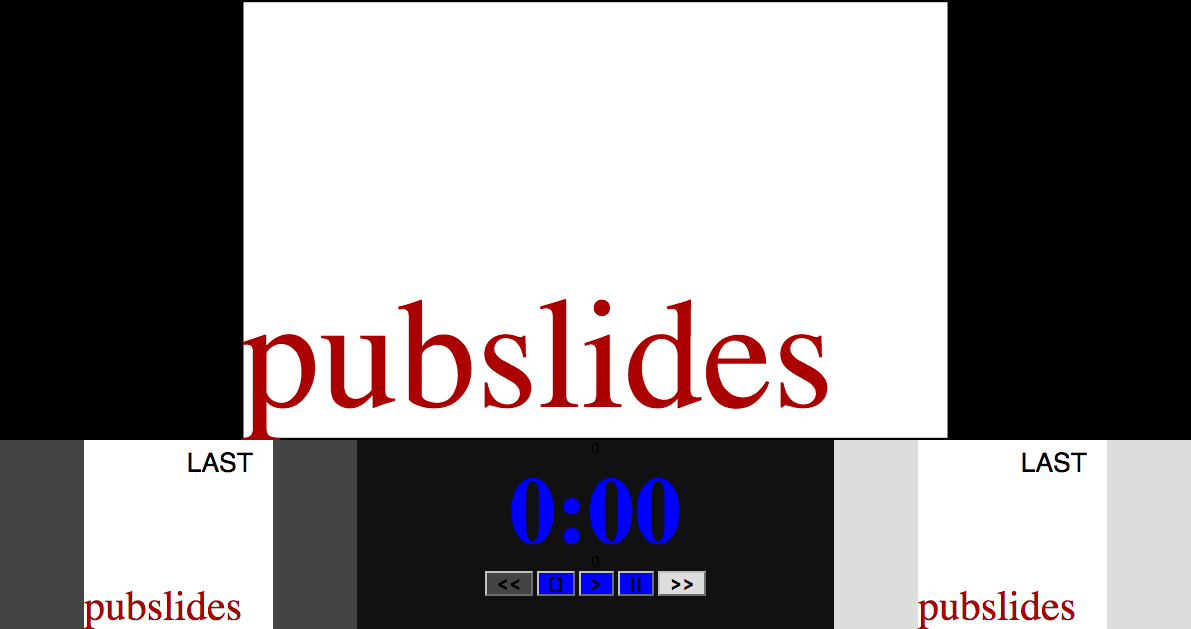
\includegraphics[width=\columnwidth]{pubslides_master}
    \caption{Master page}
	\label{fig:pubslidesmaster}
\end{subfigure}
\begin{subfigure}{.45\textwidth}
	
\includegraphics[width=\columnwidth]{pubslides_client}
	\caption{Client page}
	\label{fig:pubslidesclient}
\end{subfigure}

\caption{pubslides application pages.}
\label{fig:pubslidesapplication}
\end{figure*}


This application is currently used at the \textit{TV CompMus} page~\footnote{TV CompMus page: \url{http://compmus.ime.usp.br/en/tv}} used during the regular talks of the Compmus group.
The code of the application is available at \url{https://github.com/deusanyjunior/pubslides}.

%% ------------------------------------------------------------------------- %%
\section{Cloud Services and SuperCollider: SuperCopair}
\label{sec:appsupercopair}

The conception of \textit{SuperCopair} application happened during the period while I was an exchange student at University of Michigan.
I was interacting the live coder Sang Won Lee and noticed that few solutions are available for a distributed collaborative live coding.
After some research we discussed solutions and alternatives with Georg Essl and a the application presented in this section came out.

The \textit{SuperCopair} application was created as a package to the Atom.io~\footnote{Atom.io website: \url{http://atom.io}} IDE.
Defined as 'a hackable text editor for the 21st Century' on its site, Atom is a text editor created using web technologies and has its development powered by the github community.
This IDE has numerous packages for many programming languages and presents some solutions for coding, debugging, and managing projects.
Atom packages are programmed in CoffeeScript~\footnote{CoffeeScript website: \url{coffeescript.org}}, which is a programming language that can easily be converted to Javascript and can also integrate its libraries.
The developers can install Atom packages to enable various functionalities in the IDE such as: communicate through chats, use auto-complete in certain programming language syntax, interact with desktop and web applications, integrate with the terminal command line, and have many options based on other packages.
These features have motivated the development of SuperCopair package for Atom.

SuperCopair is based on two Atom packages: atom-supercollider and atom-pair.
The first package turns Atom.io as an alternative SuperCollider IDE and permits users to openly communicate locally with SuperCollider audio server through OSC in the same way we can do on SC-IDE.
Moreover, the users can take advantage of other Atom packages additionally to quarks packages.
The latter package is used for pair programing through the Internet.
The atom-pair package is based on Pusher cloud service and its default configuration is based on the community free plan, but a user can modify the settings and use the user’s own keys within the personal free or paid plan. 
We decided to merge both packages to add new features for collaborative live coding, and finally had dubbed it the SuperCopair package.
The main idea is that all participants have the opportunity to evolve into a collaborative performance.

The IDEs for SuperCollider have, by default, shortcuts to evaluate a line, a block, and to stop all sound process that is running.
In addition to these options, the SuperCopair package includes methods and shortcuts to broadcast these events and execute them on all users connected at the same pairing session.
Through the shortcuts, one can decide to evaluate selected code either only in the local machine, or in all computers of the session.
One can also turn on and off a broadcast alert option in the settings in order to be asked or not before evaluating every broadcast event sent by another user in the same session. This allows each individual has control over which code to be evaluated in the local machine.
The broadcast events are diffused through the cloud service and are expected to be evaluated as soon as each device receives the event message.

Networked live coding environments have been focused in collaboration.
All participants are working together to execute a musical piece and share the same final result as a common goal.
In most of the cases, sound is the only artifact that is shared, but the performers can also share codes.
Some tools enable chatting, audio, and video interaction between the participants, whether they are sharing the same physical space or they are in different locations.
Although the experiments with SuperCopair have been conducted as distributed collaborative live coding sessions, the cooperative environment has emerged during some moments.

During the sessions using SuperCopair, we had participants from different levels of experience on live coding and also some new users that decided to learn how to code during the session.
The collaboration on the final sound was similar to other live coding sessions, but the experience added another way of interaction in live coding: the cooperation. 

The cooperation aspect emerged from some events that came into view from the live coding sessions.
Experienced users are faster and have written lots of code from the scratch without any problem, while the apprentices start from basic structures or from portions of codes available on the file.
As all users were trying to synthesize the codes on all computers, it became easy to perceive if something was going wrong because everybody was sharing the code, evaluation, synthesis, and errors.
The errors coming from novice programmers were often fixed by the experienced users, and they also discussed the solutions between themselves using comments on the file.
Some tricks from the live coding practice were introduced by advanced users and the initial learners rapidly became instructors for new users and these instructors were following the same cooperative practices of the experienced users.
These events are examples of how this application can be used in many different ways: for collaborative and also cooperative performances.

A discussion about the use of cloud services for designing collaborative applications was presented during a talk in the regular Compmus seminars at IME-USP on April 6th, 2015~\footnote{Talk about cloud services: \url{http://compmus.ime.usp.br/en/node/461}}, and the discussion about the use of SuperCopair for live coding was presented August 19th, 2015~\footnote{Talk about SuperCopair: \url{http://compmus.ime.usp.br/en/node/469}}.
The code of this application is available at \url{https://atom.io/packages/supercopair} with the documentation and environment setup instructions.
The application was published as a paper at International Conference on Live Coding, Leeds, West Yorkshire, UK, in 2015~\citep{deCarvalhoJunior2015supercopair}, which is presented at Appendix~\ref{ape:papericlc2015}.
A discussion about using SuperCopair for cooperative live coding was published at Simposio Latinoamericano de Informática y Sociedad from the XLI Conferencia Latinoamericana en Informática (CLEI), Arequipa, Peru, in 2015~\citep{deCarvalhoJunior2015cooperative}, and is presented at Appendix~\ref{ape:paperclei2015}.

%% ------------------------------------------------------------------------- %%
\section{Cloud Services and Web Audio: Crowd in C[loud] piece}
\label{sec:appcrowdincloud}

An application for collaborative performance using smartphones was created with Sang Won Lee and Georg Essl while I was doing research at University of Michigan.
The main idea behind this application is that it is fully deployed on the web, the communication between devices is conducted through cloud services, and the audio synthesis is made with Web Audio API.
This combination allowed participants to join the performance using any device and any kind of Internet connection as there was small messages transmission instead of audio.

As the name of the piece suggests, the crowd (audience) plays the musical instrument in C Major. 
This is directly inspired from the piece \textit{In C}, by Terry Riley~\citep{Riley1964inc}. 
In this piece, musicians (with various instruments) were guided to play pre-composed melodic fragments in sequence for a random amount of time. 
As it is up to each musician to decide how many times to play one fragment, the collective outcome of the ensemble creates a heterophonic texture of chance.
Similarly, in \textit{Crowd in C[loud]}, each audience member plays a series of short snippets composed by herself and by other audience members.
The interface provided will first guide a participant to compose a short \texttt{``tune''} that has five musical notes in C major.

Once the participant finishes the composition, he or she can browse, and play, what other audience members have composed. 
It is thus quite similar to Terry Riley's \textit{In C}, in that one determines for oneself how long to play a tune. 
The difference is that there is no pre-composed fragments but each audience member will contribute to the piece by submitting a short melody.
In this way, participants will have their own tunes and a chord scale become the common ground upon which the entire audience plays. 
In addition, there is a separate musician performing the piece on stage at the same time with the audience members in \textit{Crowd in C[loud]}.
The role of the musician is a meta-performer who can control the chord scale in which the audience members are playing.
For example, the meta performer can, on the fly, change the instrument tuned in C major scale to a different chord scale (e.g., C Minor, Pentatonic Scale). 
This performer cannot generate sound at all on his/her end but only controls the harmonic flow of the piece as generated by the crowd.
The interplay between the musician and audience members ensures that each audience member will play individual patterns while a musician can progress the piece by changing chord scales. 
This performer-audience pairing model comes from a previous work of \textit{echobo}~\citep{Lee2013echobo} where audience members played a simplified key instrument on smartphones with the chord progression determined by a performer on stage and synchronized over a mobile network.

The performance structure was inspired by other networked pieces that presented a centralized network with a server for receiving and sending information~\citep{Weinberg2005interconnected}.
However, our choice of using the Pub Nub cloud service set us free from the burden of developing a custom server application, which is replaced with a single web page written in HTML and Javascript.
This will be a useful setup for artists who want to write a network music piece who do not have a networking background but can write an interactive web page.
PubNub cloud service permits easy interconnection between users through channels using publish-subscribe (or pub-sub paradigm).
An application~(or device) can subscribe to a channel and receive every notification that is published to the channel. 
For example to broadcast a message to all devices, a device can publish a message to a channel that every device is subscribed to. 
This provides a convenient abstraction that is robust against changes in network or end-user device and allows dynamic reconfiguration of participation.
The push(or publish) notifications paradigm also makes performances more robust against technical disruptions such as disconnection and delays.

The left side of Figure \ref{fig:performance} presents the performance setup at the concert hall.
There were two kinds of web pages running during the performance, one for the performer and another for the audience.
The performer sat center-stage and his application (a web page) was project onto a screen for the participants seated in the audience.
They were instructed to visit their application that has the musical instrument on.
The performance hall had wireless network available from the university and had a good reception of mobile network connectivity such as 3G.

A representation of the cloud service with the channels we used is on the right side of the Figure~\ref{fig:performance}.
In our performance we designed three types of channels following the PubNub API for web application: a performer channel, an audience channel and individual channels equaling the participant number. 
The performer application is subscribed to the performer channel to receive messages sent from audience member's devices. 
Once a participant visits, it requests a performer's application to create an individual channel by publishing a message to the performer channel.
The individual channel is then created to respond to an audience application's request, typically for the audience to retrieve a tune composed by others.
When the page is loaded, every device is given a universal unique identifier (UUID) from the cloud service API, which is used to create an individual channel.
Lastly, all the audience members are subscribed to the audience channel. 
This channel is used for crowd control: to send textual instructions, to live-code the mobile instrument, to start/end the performance and to troubleshoot the performance when it goes wrong (silence, refreshing the page).

\begin{figure}[t]
	\centering
	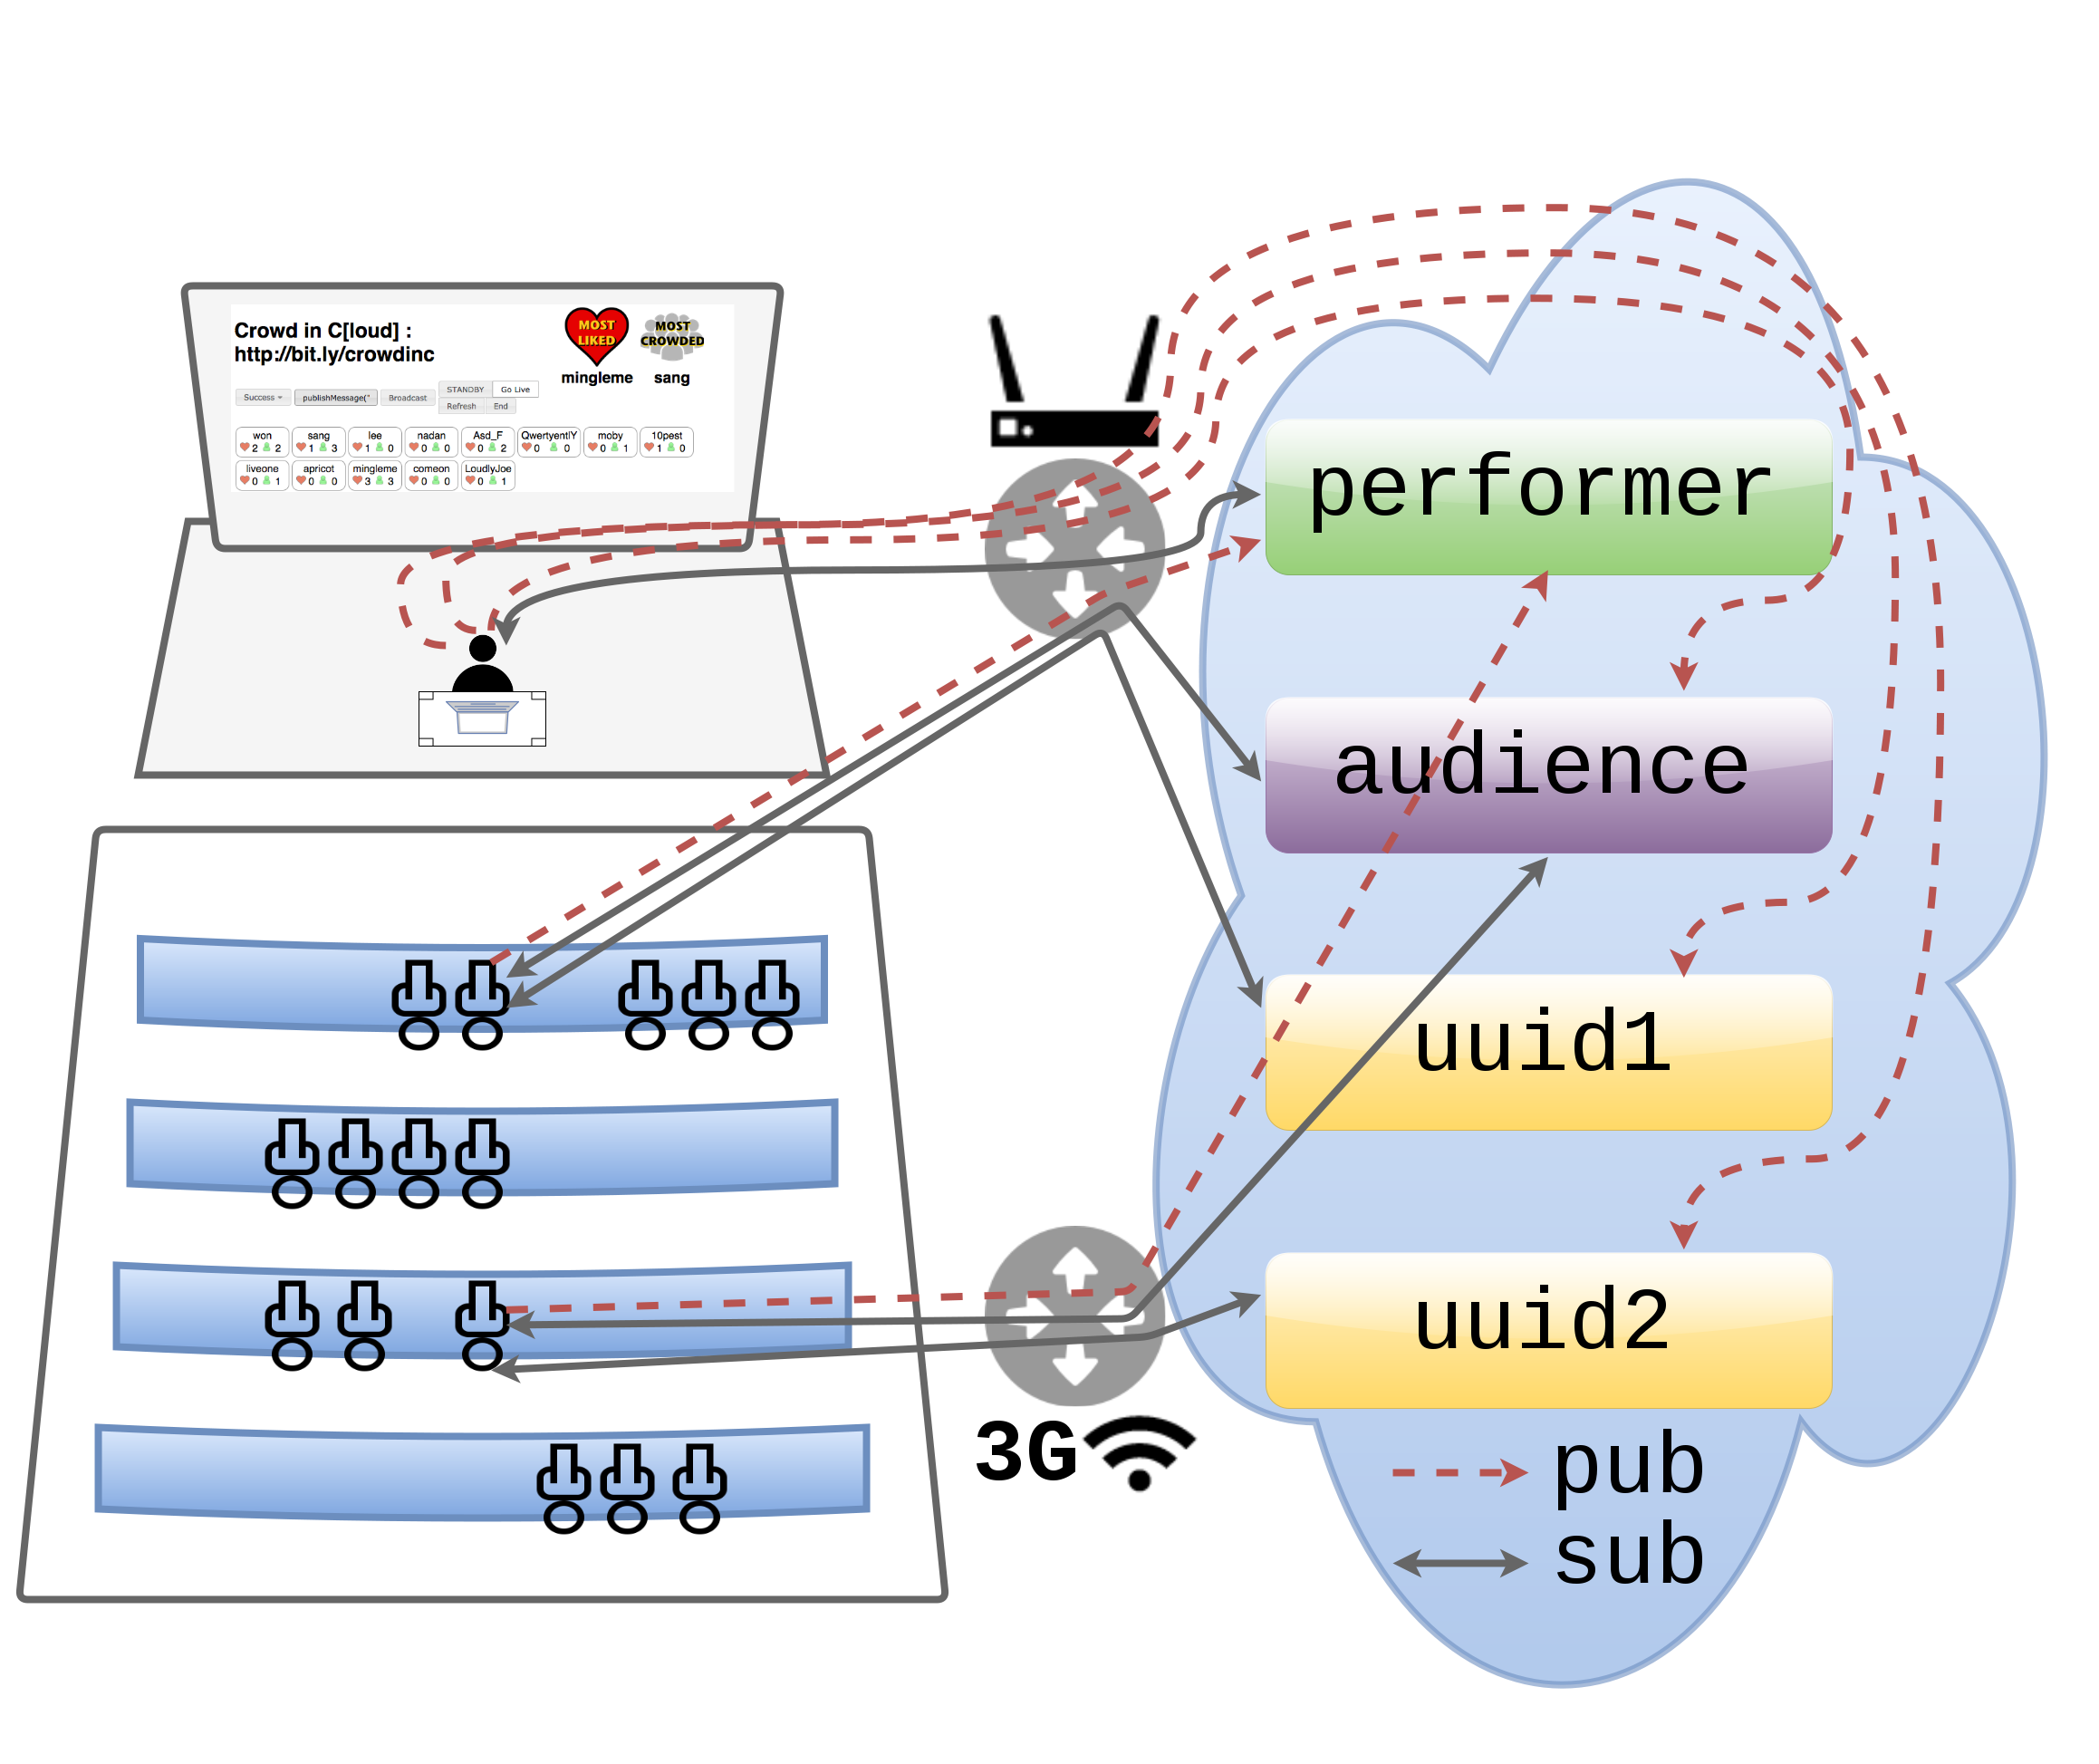
\includegraphics[width=0.5\columnwidth]{performance}
	\caption{Performance structure. The left side depicts the performance space. On the right side, a rectangle represent a channel, solid lines show publishing and dotted lines show subscription.}
	\label{fig:performance}
\end{figure}

\textit{Crowd in C[loud]} was performed at many venues during the past two years and the debut happened on April 18, 2015 in Stamps Auditorium at the Walgreen Drama Center on the U-M North Campus~\footnote{Debut of \textit{Crowd in C[loud]}: \url{http://www.eecs.umich.edu/eecs/about/articles/2015/w15-mobile-phone-ensemble-performance.html}}.
The video from the debut is available at \url{https://www.youtube.com/watch?v=8RWgXoM2BCA} and a multi-camera video of a performance in Atlanta is available at ~\url{https://www.youtube.com/watch?v=8nnrKJ4Ap0c}.

The discussion about sound synthesis was published as a paper in 2nd Web Audio Conference (WAC), Atlanta, Georgia,  USA, in 2016~\citep{Lee2016crowd} and the discussion regarding network communication through the cloud services was published in the 16h International Conference of New Instruments for Musical Expression, Brisbane, Australia, in 2016~\citep{deCarvalhoJunior2016understanding}.
The papers published in these conferences are presented in Appendix~\ref{ape:paperwac2016} and Appendix~\ref{ape:papernime2016}, respectively.
A discussion about the application was presented during a talk in the regular Compmus seminars at IME-USP on September 16th, 2015~\footnote{Talk about Crowd in C[loud]: \url{http://compmus.ime.usp.br/en/node/475}}
The code used on the application is available at \url{https://github.com/panavrin/tindermusic}.

%% ------------------------------------------------------------------------- %%
\section{iOS, Lua, and Network communication: Performances with urMus}
\label{sec:appsumich}

The final projects of the course audited at University of Michigan resulted in musical performances.
One of the performances that I participated during the conception was \textit{Crowd in C[loud]} presented in Section~\ref{sec:appcrowdincloud}.
Two other performances described below were based on mobile applications created using the \textit{urMus} platform.
Both performances used a similar approach regarding the network communication inside the platform using the Lua language.

Although the \textit{urMus} supports OSC, listening to OSC messages through a specific IP is unavailable so then the Multicast communication was discarded.
The technology used in this case was the Bonjour methods for network advertising and discovery.
The master device was configured to discover all other devices advertisements.
Every discovered device is attached to a list of available devices and the master device can use this list to send messages to all devices in this situation.
This approach was evaluated for different numbers of devices and the more devices we added the more the application was overloaded with the network communication.
The solution is similar to the Multicast algorithm available in many routers and the code is presented at Listing~\ref{urMusLuaMulticast}.
The pieces are described in the next sections.

\begin{footnotesize}
\lstset{language=Java, caption=Example of Lua code used at urMus platform for Multicast networking simulation, captionpos=b, label=urMusLuaMulticast, numbers=none, numberstyle=\scriptsize}
\begin{lstlisting}[frame=single]
local myIP, myPort = HTTPServer()
endPoint = string.find(myIP, '.', string.find(myIP,     '.',string.find(myIP, '.',1, true)+1, true)+1, true)
local ownId = tonumber(string.sub(myIP, endPoint+1))

local function NewConnection(self, name)
	DPrint("new friend "..name)
	DPrint("")
	for j,u in pairs(friends) do
		if u == name then
			return
		end
	end
	friendEndPoint = string.find(name, '.', string.find(name, '.',string.find(name, '.',1, true)+1, true)+1, true)
	friendId = tonumber(string.sub(name, friendEndPoint+1))
	table.insert(friends, name)
	friendsKey[friendId] = table.getn(friends)
end

local function LostConnection(self, name)
	for l,w in pairs(friends) do
		if w == name then
			table.remove(friends,l)
		end
	end
end

function sendNote(noteToSend)
	DPrint("sent "..noteToSend)
	DPrint("")
	for indexIp = 1, table.getn(friends) do
		local ip = friends[indexIp]
		SendOSCMessage(ip,8888,"/urMus/numbers",noteToSend, ownId, currentPage)
	end
end

function gotOSC(self, noteReceived, senderId, senderPage)
	DPrint("got osc")
	DPrint("")
	if senderPage == 3 then
		addPoints(senderId)
	elseif senderPage == 2 then
		createNote(keysP[noteReceived])
	end
end
...
StartNetAdvertise("ttss",8889)
StartNetDiscovery("ttss")
...
SetOSCPort(8888)
host, port = StartOSCListener()
\end{lstlisting}
\end{footnotesize}

%%%%%%%%
\subsection*{Twinkle, Twinkle Smartphone Star}

This performance was conceived in a partnership with Zachary Boulanger and the concept is related to playing with the idea of expectations. 
The master performer would be a composer using the master application with an 8-key keyboard that was configured to send every key touched to all the friends available.
The other performers would have the same keyboard and they would receive the information regarding the notes to be played.
Each note was converted to falling balls over the keyboard keys and the performers were invited to touch the correspondent key as soon as the ball reaches the other side of the screen.

On the performance conception, the composer expects the performers to play his creation exactly right, however the players soon realize they are not bound to this.
The audience expects to hear well-known canons and to hear the music ``written'' by the composer, but once the performers start changing it up these expectations are broken.
While composer is creating melodies based on canons, the audience will see the notes coming from the top of the projector screen and they are expected to hear the notes once they reach the bottom. 
In the beginning the performers will play only their specific notes, but some of them are going to try other notes and the perception of the melodies will diverge from the reality. 
As the performers decide to walk on the stage, it will became hard to know who is expected to play the right note.

The audience will expect some control from composer hands, but he is using a headphone and will not hear anything. 
In the middle the composer will take out the headphone, he will try to control the performers again, and stop sending notes to the end the piece.
The sound experience comes from the idea that the audience will expect some melodies based on the notes that are falling down, but it doesn't depend only on the composer's composition, because the composer is not a player.

%%%%%%%%
\subsection*{Himalayan Singing Bowl}

Biqiao ``Didi'' Zhang was the composer of this piece and I participated with Zachary Boulanger as partners during the development of the mobile application.  
In this piece we simulate a himalayan singing bowl through multiple mobile devices. 
One person is the ``conductor''/``leader'' of the performance and this person controls which note the devices are playing (e.g. C3) and how people should be moving their devices. 
Ideally, only the performers know who the leader is.
The performers will all be standing in a circle on stage, facing inward. 
They move their devices up and down to control the volume and left and right to control the ``beating'' of the sound. 
The color on their screen changes with their movement. 
A projector displays a video of a singing bowl, so the audience knows what the performance is based on.

The difference in frequencies by each performer, their place on the stage, and the changing color of the screen mimicking their movements all provide a unique spatial element to the performance. 
The absence of a clearly defined conductor also lends to the idea of circular performance with everyone following everyone else’s movements and actions. 
This shows that the performance not only simulates the singing bowls musically, but in a physical aspect as well.
The sound is simulating an actual singing bowl, with the performers forming the bowl itself. 
Each person has a different frequency than those next to them, giving a spatial element to the musical experience. 
The performance is then made more musically interesting with the addition of different pitches, dynamics, and ``beating''. 
This is where our simulation grows and differs from the original, making the performance something new entirely.

These performances were performed on April 18, 2015 in Stamps Auditorium at the Walgreen Drama Center on the U-M North Campus~\footnote{Performances with urMus: \url{http://www.eecs.umich.edu/eecs/about/articles/2015/w15-mobile-phone-ensemble-performance.html}}.
The videos from these performances are available at \url{https://www.youtube.com/watch?v=8RWgXoM2BCA}.


%% ------------------------------------------------------------------------- %%
\section{Web Audio versus Audio Samples: Contribution to Open Band}
\label{sec:appbandaaberta}

Two researchers from NuSom group and Compmus created a performance named ``Open Band'' using many web technologies.
The concept behind this performance was to create an online webchat and allow users to exchange messages publicly without nicknames or identification.
The first version of this performance had a web page that converted letters into sounds and used audio samples.
Although the performance was conceived to local networks, they were using a high number of audio samples, with 30MB of size.
I attended some of their presentations and noticed that the performance was too heavy for mobile devices and the server could be overloaded depending on the number of participants considering that all participants were retrieving the audio samples from the server at the same time.

After some discussions, I decided to participate in a new version of the performance but changing some technologies.
The current version of the ``Open Band'' is now entirely based on web audio synthesis and reduced the bandwidth requirements for the audience participation.
This upgrade to the performance removed the restriction for performing in local networks and the system used can now be deployed on web servers.

During the development of this new version we opted to evaluate some ready-made solutions for web audio synthesis like Gibber~\citep{Roberts2012gibberlivecoding}, Waax~\citep{Choi2013waax}, and meSpeak.js~\footnote{meSpeak.js website: \url{http://www.masswerk.at/mespeak/}}.
These solutions are able to facilitate the use of web audio technology and other browser facilities, but also create barriers and sometimes limitations that are not imposed by pure web audio.
Furthermore, sometimes frameworks could offer more than what was required by the application, which can lead to more confusion during development. 
We tried to use, meSpeak.js as a simple and interesting text-to-speech library but the resulting sound was not musically satisfactory, and the framework limited messages to play on top of each other.
The current version focus on pure web audio for sound synthesis and we also decided to follow some aesthetic concepts based on phonetic and audio typography, to experiment with new kind of music, avoiding traditional chords and scales. 
These concepts surrounded the whole development of this new version of ``Open Band'' and had a great impact in the new result obtained.

The code of the current version of the application used during this performance is available at \url{https://github.com/fabiogoro/banda/tree/master/bandawa}.
We submitted a full paper to the 3rd Web Audio Conference~(WAC) that will be held in the end of August, 2017 at the Centre for Digital Music, Queen Mary University of London.
The submitted version of this paper is available at Appendix~\ref{ape:paperwac2017}.
